% ALICE COMMENTS---
% EMAIL 1:
% General observations- Tritium breeding and power density should also be included in your vocabulary 
% Insert a picture of pebble bed before 1.2 (or move Fig. 1.3 to there)
% Specific sentences: 
% 1) DONE -- Thus to provide designers the ability to optimize breeder volumes for "tritium breeding and subsequent" tritium release,
% 2) DONE -- In this approach, heat transport in pebble beds is often characterized with an effective thermal conductivity, keff,  "and interface heat conductance"
% 3) DONE -- and considerations of "slow moving" inter-porous helium purge gas.
% Question
% Have you showed "and changes to bed stresses and contact-force networks in beds with restructured packing" in the past? 


%%%%%%%%%%%%%%%%%%%%%%%%%%%%%%%%%%%%%%%%%%
\chapter{Introduction} \label{sec:introduction}
%%%%%%%%%%%%%%%%%%%%%%%%%%%%%%%%%%%%%%%%%%
% brief intro of pebble beds
Helium-cooled pebble beds (HCPB) of lithium ceramics exist in candidate designs of tritium breeding devices of many current nuclear fusion demonstration reactor designs as well as tritium breeding modules to be tested in the ITER experiment. HCPBs will be used to generate high quality heat for electricity production and breed tritium for a self-sustained fuel cycle. Pebble bed forms of tritium breeding volumes have several advantages which include: ease of assembly of granular materials into complex geometries; bred tritium can be readily removed via a helium purge gas through interstitial porous networks; temperature gradients across any single pebble are small enough to avoid damage from thermal stress. 

A relatively narrow operational temperature window for optimum breeding performance of ceramics must be observed to respect temperature-dependent phenomena driving tritium release from lithiated ceramic pebbles. It is therefore necessary to have accurate knowledge of ceramic pebble bed thermomechanical behavior and comprehensive characterization; reliable models of heat transfer in solid breeders are critical for solid breeder designs. However, temperature prediction in ceramic pebble beds remains a challenge for many reasons. After packing the ceramic pebbles into a containment structure, there exists a coupling between mechanical forces acting upon beds and their heat transport capabilities. In addition, some amount of restructuring of the pebble bed and the internal contact force network is likely to occur in HCPBs from crushing/cracking of individual pebbles, inter-pebble sintering, or creep during operation. Contact conduction in beds, intimately linked to the packing structure, will subsequently be impacted during operation of ceramic pebble beds in fusion reactors. Concurrently, interaction of the slow-moving purge gas with tightly packed pebble beds is an additional route of heat transfer that must be understood. Thus, heat transfer in pebble beds is quite different from standard solid materials and requires specialized modeling of the synergistic physics. Knowledge and characterization of thermal transport must anticipate changes to the heat transfer capabilities and predict temperature profiles for pebble bed packing structures that will emerge after initially-packed pebble beds react to prolonged exposure to fusion reactor environments.

In the remaining sections of this chapter I will present more background on the role of ceramic pebble beds in tokamak fusion reactors, more thorough descriptions of solid breeder blanket designs, and the objectives of this study.


















\section{Description of Ceramic Pebble Bed Designs for Tritium Breeding}
\begin{figure}[ht]
	\centering
	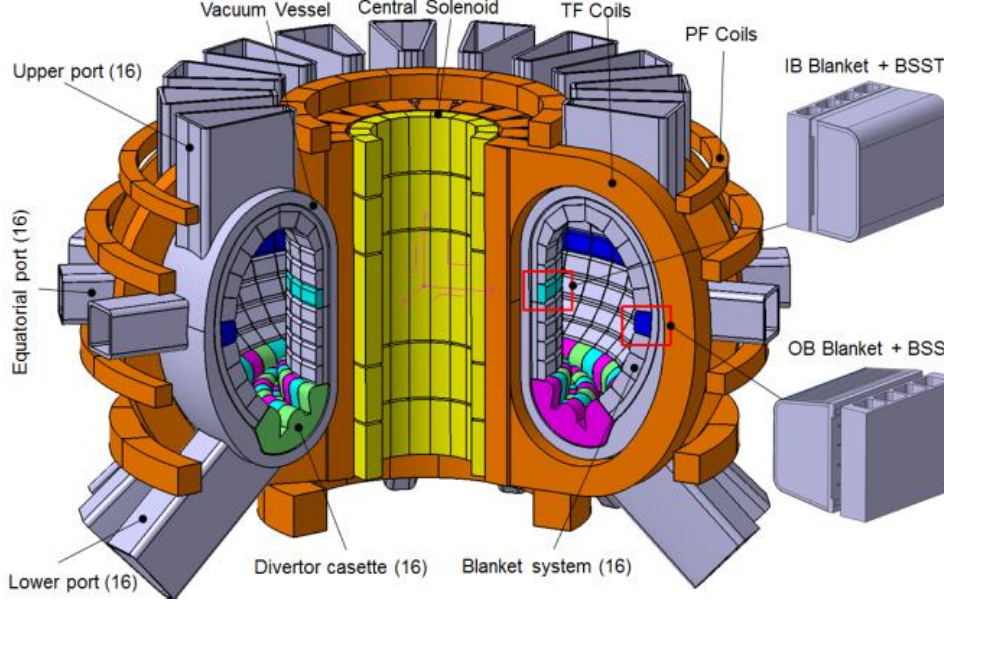
\includegraphics[width=\singleimagewidth]{figures/demo} 
	\caption{An example design of a DEMO reactor with solid breeder blankets shown as inboard (IB) and outboard (OB) blanket components.}
	\label{fig:demo}
\end{figure}


% stole this from Zhiyong.  UPDATE
The fusion reactor as a promising energy supplier has been intensively studied for decades. The economic, safety, and environmental attractiveness of fusion reactors will be determined, to a large extent, by the choice of materials for the performance of the blanket. Specifically, for a solid breeder blanket concept, issues such as the thermomechanics of solid breeder materials and irradiation effects on tritium release characteristics remain to be addressed in more detail. %The breeder blanket is a critical piece of engineering technology upon which the success of a fusion power plant largely rests. 
% /stole this from Zhiyong.  UPDATE

The successful operation of a breeder unit will see the device capture neutrons ejected from the fusion reaction to generate fuel for self-sufficiency via the transmutation of lithium into tritium, act as shield to other sensitive equipment and personnel, and convert energy into extractable heat for electricity production. \Cref{fig:demo} shows an example sketch of a demonstration (DEMO) fusion reactor and the relative location of the breeder blanket modules as they will face the plasma in the torus of the tokamak. %The solid breeder is one proposed design. Other design concepts see lithium, in liquid form, flowing through the breeder module and then into the fuel processing cycle. These so-called liquid breeders are an entire field of research in their own right and are not discussed in this work.

Since the inception of the solid breeder concept in the late 1970s, designs have evolved in response to operational requirements of harsh fusion reactor environments. Currently, the reference solid breeder design incorporates packed beds of ceramic pebbles (spherical particles) that are filled into containment structures. In a typical solid breeder module, the breeding volume is subdivided into several alternating layers of neutron multiplication material (generally beryllium) and tritium breeding material. The layers are separated by coolant plates with internal channels for coolant. The coolant is typically a high pressure helium though some designs call for pressurized water, in spite of the dangers of the highly exothermic reaction with oxygen from water vapor and lithium in the case of coolant leak. After a neutron strikes lithium for the creation of tritium, the bred hydrogen isotope diffuses through the ceramic material until being picked up by a low-pressure, slow moving purge gas (primarily helium) and extracted in a closed loop for fuel.


\section{Solid Breeder Thermal Management and Imposed Temperature Window}

\begin{figure}[ht]
    \centering
    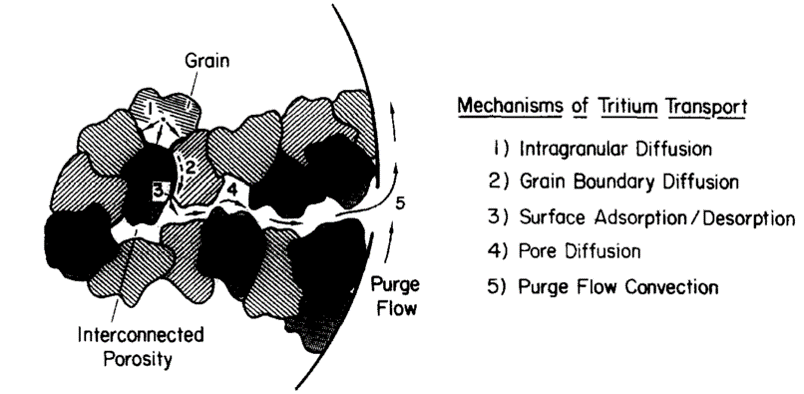
\includegraphics[width=\singleimagewidth]{figures/mechanisms_tritium_transport} 
    \caption{Mechanisms of tritium transport in a single pebble\cite{Federici1990}.}
    \label{fig:mechanisms_tritium_transport}
\end{figure}

To understand the importance of predictive capabilities of temperature in solid breeders, we first consider one of the main roles of the breeder is to readily allow tritium to be extracted. Therefore we can first consider the path of tritium from its generation until it is swept away by the helium purge gas; the journey of tritium is shown schematically in \Cref{fig:mechanisms_tritium_transport}. Tritium begins its life internally inside pebbles. Tritium then diffuses slowly through the bulk of the ceramic lattice until reaching a grain boundary. At this point, tritium diffuses more quickly along the grain boundary until reaching a surface of open porosity where it may desorb into stagnant gas in a pebble's open porosity. Finally, tritium diffuses more rapidly still through the gas until being swept up in the advection of helium purge gas.\cite{Federici1990} 

Experiments on tritium inventory have attempted to quantify the speeds of tritium release and found that bulk diffusion of tritium, typically the slowest transport mode, is a direct function of temperature.\cite{Franza2013} Thus the lower temperature limit, $T_\text{min}$, of temperature windows for solid breeders, is based on the unacceptable tritium inventory due to slow bulk diffusion. The value of $T_\text{min}$ is generally around \SI{300}{\celsius}. Using the same model of tritium transport, bulk diffusion also limits the maximum temperature in the solid breeder temperature window. Exposure to prolonged high temperature environments causes individual grains in a pebble to grow. Grain growth therefore extends the characteristic length of the slowest mode of tritium transport. Thus the maximum temperature, $T_\text{max}$, of the operational window for ceramic pebble beds is generally placed around 80\% of the melt temperature of the ceramic, $T_\text{max} = 0.8 T_\text{melt}$, to avoid surface sintering. For many lithium ceramics, this value falls around \SI{900}{\celsius}.

As a consequence of the tritium release from the solid breeder material, we are faced with a relatively narrow operational temperature to which solid breeder designers must adhere. Thus to provide designers the ability to optimize breeder volumes for tritium breeding and subsequent tritium release, we must understand the important physics and phenomena dictating thermomechanical responses of pebble beds during use in a fusion reactor.


\begin{figure}[ht]
	\centering
	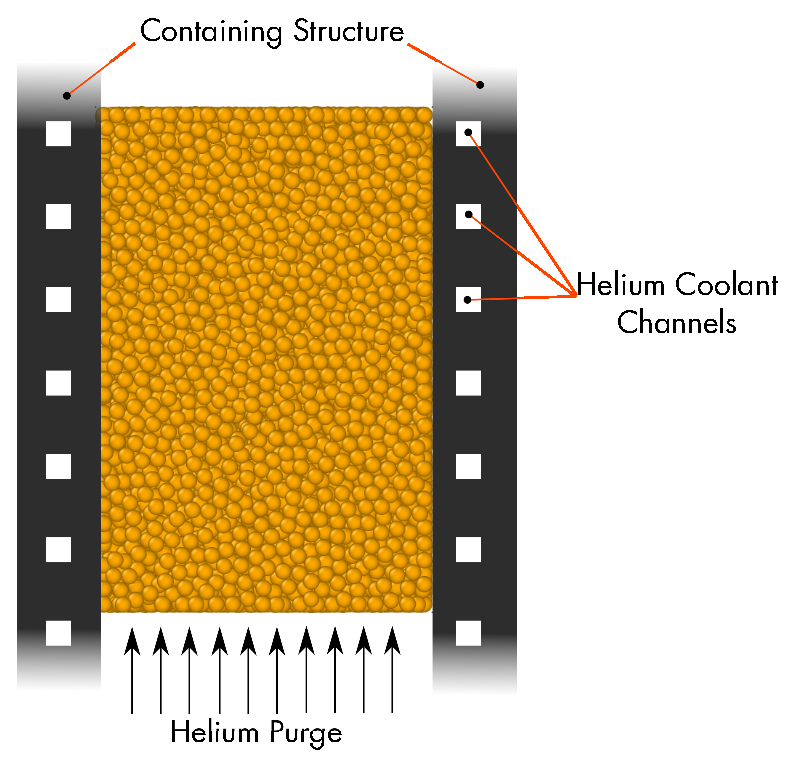
\includegraphics[width=\singleimagewidth]{figures/solid_breeder_sketch} 
	\caption{Sketch of a typical unit of a pebble bed tritium breeding zone. The pebble bed is cooled with contact to the containing structure.}
	\label{fig:solid-breeder-sketch}
\end{figure}

% High energy (14 MeV) neutrons are ejected from the deuterium-tritium reaction, as described by \Cref{eq:dt-reaction}
% \begin{align}
%     \mathrm{D} + \mathrm{T}&\xrightarrow{}\ ^4\mathrm{He}+\mathrm{n}+17.58\ \text{MeV} \label{eq:dt-reaction}
% \end{align}
% thus t

\Cref{fig:solid-breeder-sketch} shows a generic solid breeder volume that is common in current designs of tritium breeding modules for ITER. Tritium breeding blankets will experience high volumetric heating as deposited by high-energy neutrons that are carrying away approximately 80\% of the fusion reaction energy as well as secondary $\gamma$ rays. The deposited heat must be transported through the pebble bed region into the walls of the containing structure, then ultimately into the coolant gas. Heat deposited into pebble beds will transfer via inter-particle contact conduction, inter-particle radiation, and convection with the helium purge gas. At the interface with the structural material, similar modes of heat transfer are present: particle-wall contact conduction, particle-wall radiation, and communication via helium purge gas convection. As the pebbles heat under the nuclear load, thermal expansion of the pebbles in the packed volume will be contained by relatively cooler structural material. Confined expansion will give rise to increased contact pressure between pebbles. Pressure on pebble beds is known to be the cause of many phenomena, some of which directly impact the thermal transport characteristics of pebble beds and may ultimately jeopardize the reliable and safe operation of breeding blankets. 

The packing structure of packed beds can be considered as a metastable configuration that will last indefinitely unless acted upon by an external perturbation such as vibration or compressive pressure.\cite{Jaeger1996} The ability of a metastable configuration to resist perturbations can in some way be quantified by the initial packing fraction. For more compliant beds, with lower packing fractions, the stresses from thermal expansion can cause significant rearrangement of the packing structure which is not recoverable after removing the stress. This phenomena has been observed in numerous experiments as so-called plastic rearrangement of pebble beds.\cite{Reimann:2002kl,Reimann:2000tw,Zhang2015} Plasticity of beds may have significant consequences for the ability of the pebble bed to maintain contact with the containing structure and routes for heat out of the bed due to gap formation between the two materials. Moreover, increased pressure between pebbles can cause the brittle pebbles themselves to fragment which will also disrupt paths of heat in the inter-particle conduction network. The consequence of both the mentioned effects is an increase in the temperature of bed pebbles. If the fragments are sufficiently small, they may even cause blockage of the helium purge gas. 

Due to the complicated nature of granular materials such as ceramic pebble beds, heat transfer in these solid breeder volumes should not be considered as a static phenomena that can be characterized prior to inserting pebbles beds into breeder modules and then expected to behave consistently after long exposure to fusion environments. Pebble bed temperatures, linked to the packing, will evolve in ways that are currently not predictable and must be studied and modeled.

In spite of their many engineering applications, heat transfer mechanisms in packed beds of granular material are still not thoroughly understood nor characterized. Hence, one approach is to treat the granular material as a fictitious continuous media, an approach adopted by several designers of solid breeders. Many experiments have been carried out for developing phenomenological models for effective material properties. In this approach, heat transport in pebble beds is often characterized with an effective thermal conductivity, $\keff$, and interface heat conductance. Many models have shown their ability to accurately predict the temperature profiles for pebble beds under specific operating conditions. However, the accuracy of the model predictions often degrade as soon as a pebble bed's granular material, grain radii distributions, or operating conditions vary from the experimentally studied packed beds. In addition, propensity for creep, crushing, and inter-particle sintering of ceramic materials alter the packing structure in ways not currently predictable with the effective material characterizations. Furthermore, effective conductivity models that consider interstitial gas often assume the gas is stagnant. The assumption has not been thoroughly vetted and is likely insufficient to capture the thermal influence of the helium purge gas flowing through the ceramic pebble beds in fusion reactors.

To overcome the limitations of effective material modeling, and aided by the acceleration and availability of computational power, many researchers of granular heat transfer have shifted their attention to studies of the interacting physics on grain-scales. In this approach, we interrogate heat transfer on the scale of particle interactions and model transient, grain-scale behavior in packed beds. We can then couple grain-scale models of heat transfer and mechanics to either volume-averaged fluid models or models of the entire tortuous fluid flow through the porous network of packed beds.
note: have to mention that i'm using DEM I guess. maybe in the objectives section?

\section{Objectives of this Study}\label{sec:intro-scope-of-work}
% from the intro originally, fit this in with the paragraph below.
The goal of this work is to develop more comprehensive and accurate models for predicting temperature distributions in ceramic pebble beds, accounting for many important phenomena including pebble crushing and fragmentation, dynamic analysis of packing restructuring, and considerations of slow moving inter-porous helium purge gas. In particular I will study in great detail the relationship between morphological changes to packing structures and the resulting changes to heat transfer in packed beds. In particular, I will be concerned with the nuclear heating of pebble fragments as they redistribute through pebble beds and come to rest without strong mechanical contact (and therefore contact conductance) to neighboring pebbles. This includes analyzing changes to temperature distributions in pebble beds with different models of pebble damage, analyzing the impact of helium flow on temperatures in beds with fragmented pebbles, and changes to bed stresses and contact-force networks in beds with restructured packing. Experimental efforts will inform numerical development at the start. Following, numerical model development and application and extensive data analysis will be the main approach taken in this study. Satisfying the objectives of this work includes several major efforts that can be summarized as follows:

Experimental campaigns crushing various lithium ceramic pebbles (\lit and \lis) between two nickel-based steel alloys will be carried out at temperatures ranging from room temperature to \SI{650}{\celsius} to observe the temperature-dependence of crush strength. From the experimental data, I will also validate the Hertzian assumption for contact mechanics of the spherical pebbles on the flat pistons; experiments measure the force-travel response of individual pebbles and, via comparison with predictions of Hertz theory, will show a modified Young's modulus is necessary for use in the material inputs. The crush experiments will also be used as a basis for developing a criteria for prediction of pebble crushing in packed beds. 

Numeric campaigns will develop in stages. In the first stage, many components of the pebble bed modeling will be tested individually. Simulations strictly of heat transfer dependence on pebble interactions (without consideration of fluid flow) will be executed to analyze the links between pebble descriptions (\textit{e.g.} packing fraction, coordination number, contact forces) and temperature distributions in pebble beds with specific models of pebble damage. A study will apply the modified Young's modulus model to show the dependence of crush predictions and external measured stresses of beds on the Young's modulus assigned to pebbles in simulations. Finally, another separate study will assess the impact of fragment size on packing resettling and its role in thermal transport.

In the second stage, pebble beds similar to the first stage will be analyzed, with and without helium flow. In this stage, the helium flow will be two-way coupled to the pebble bed with fluid phase being characterized with volume-averaged conservation equations. We will see the role of helium on smoothing out temperatures between pebbles which have poor mechanical contact with neighbors in the assembly. Again, effective thermal conductivity measurements will be reported from well-packed beds and beds with pebble damage. Lastly, in this stage, several ITER-relevant configurations of pebble beds are studied. 

In the third stage, pebble beds are one-way coupled to models of helium flow. Rather than considering volume-averaged conservation equations, we will make use of the novel approach of solving lattice-Boltzmann equation on discretized lattice nodes which allow for simple application of boundary conditions on the complex geometry of packed beds. This approach will provide a more complete view of helium's serpentine route through the pebble bed and its impact on temperature distributions in beds.



%A more thorough understanding of temperature distributions allows for higher confidence in tritium release from pebble beds as well as the potential for increased power density during operation of the solid breeders. 

% One last note: there are other long-term effects expected in the materials experiencing prolonged exposure to cycling irradiation, heat, and stress that have not been discussed here. These loads can lead to thermal ratcheting, irradiation swelling, sintering, or thermally-induced creep which also lead to evolutions in thermophysical properties -- even in the absence of cracked pebbles. These phenomena need to be addressed in time but are, however, beyond the scope of this dissertation. 
\section{Dissertation Outline}
In the next chapter I will present a literature review on the state of the art of modeling granular materials and packed beds, including: effective thermal conductivity experiments and their derivative empirical relationships, convective energy exchange in packed bed media, and drag of fluid flow through packed beds. The literature review also discusses the specific application of granular research for packed beds in the fusion community, highlighting progress made and where deficiencies in research remain. In \Cref{ch:modeling-development}, I will present the theory behind the discrete element method modeling for granular interaction as well as experimental efforts to validate Hertz theory and aid in development of pebble damage modeling. Then \Cref{ch:cfd-dem-modeling-development} covers the coupling of the pebble model in DEM to the volume-averaged CFD as well as coupling to solvers of the lattice-Boltzmann equation. After model development is complete, in \Cref{sec:dem-studies}, I begin application of the models to study of temperature distributions in ceramic pebble beds for tritium breeding; first models are run only in the DEM environment, then with the coupled CFD-DEM models, and finally with coupled DEM-LBM simulations. Finally in \Cref{sec:summary} a summary of the work, the impact of the results, and a suggestion for future work will be presented.